\documentclass{article}
\usepackage{arxiv}
\usepackage[utf8]{inputenc}
\usepackage[english, russian]{babel}
\usepackage[T1]{fontenc}
\usepackage{url}
\usepackage{booktabs}
\usepackage{amsfonts}
\usepackage{nicefrac}
\usepackage{microtype}
\usepackage{lipsum}
\usepackage{graphicx}
\usepackage{natbib}
\usepackage{doi}


\title{Классификация товаров по ОКПД2 кодам}

\author{ Фирсов Сергей Андреевич\\
        Кафедра интеллектуальных систем\\
	МФТИ\\
	\texttt{firsov.sa@phystech.edu} \\
	\And
	Старожилец Всеволод Михайлович  \\
	Кафедра интеллектуальных систем\\
	Форексис\\
	\texttt{vsevolod.starozhilets@antirutina.net} \\
	\AND
	Вознюк Анастасия Евгеньевна \\
	Антиплагиат \\
        МФТИ \\
        \texttt{vozniuk.ae@phystech.edu} \\
	%% \And
	%% Coauthor \\
	%% Affiliation \\
	%% Address \\
	%% \texttt{email} \\
	%% \And
	%% Coauthor \\
	%% Affiliation \\
	%% Address \\
	%% \texttt{email} \\
}
\date{}


%%% Add PDF metadata to help others organize their library
%%% Once the PDF is generated, you can check the metadata with
%%% $ pdfinfo template.pdf
\hypersetup{
    colorlinks=true,
    linkcolor=blue,
    filecolor=magenta,      
    urlcolor=cyan,
    pdftitle={Overleaf Example},
    pdfpagemode=FullScreen,
    pdftitle={Классификация товаров по ОКПД 2 кодам},
    %pdfsubject={hierarchical classification, embeddings, logarithmic regression},
    pdfauthor={Фирсов Сергей, Старожилец Всеволод, Вознюк Анастасия},
    pdfkeywords={hierarchical classification, embeddings, logarithmic regression},
}

\newcommand{\customcite}[2]{\footnote{#2, see \cite{#1}}}
\bibliographystyle{plain}

\begin{document}
\maketitle

\begin{abstract}
    Исследование направлено на решение задачи классификации товаров по кодам Общероссийского классификатора продукции по видам экономической деятельности (ОКПД 2) с использованием кратких текстовых описаний. Коды представляют собой детализированную систему категоризации продуктов и услуг по видам экономической деятельности. Основная цель --- повышение точности и сокращение ресурсозатратности классификации, за счёт анализа влияния глубины ОКПД 2. Для достижения этих целей предлагается метод построения текстовых эмбеддингов. Задача усложняется необходимостью предварительной обработки данных для перевода исходных описаний в стандартизированные короткие тексты, адаптированные для анализа. Используются данные государственных закупок по ФЗ 44 за 2022 год. Новизна работы заключается в применении методов машинного обучения к индустриальной задаче, что обещает улучшение в процессах логистики, учёте и анализе в сфере закупок. 


 
\end{abstract}


\keywords{OKPD 2 code \and text analysis \and multiclass classification \and embeddings\and logarithmic regression}

\section{Введение}

Целью данного исследования является разработка и апробация метода классификации товаров по кодам ОКПД 2\footnote{Общероссийский классификатор продукции по видам экономической деятельности, \href{https://classifikators.ru/okpd}{сайт}}, используя краткие текстовые описания. Основная идея заключается в построении эмбеддингов и дальнейшем решении задачи многоклассовой классификации. Актуальность задачи обусловлена необходимостью повышения эффективности процессов логистики и учета в сфере закупок, а также сокращения времени и ресурсов, затрачиваемых на классификацию товаров. \textit{(тут нужна прямая ссылка где требуется, но у меня индустриальная задача, которая буквально дана как нужная в фирме Всеволода Михайловича )}

\textbf{Основные термины}:
\begin{itemize}
    \item ОКПД 2 (Общероссийский классификатор продукции по видам экономической деятельности) -- система классификации, используемая для каталогизации продукции.
    \item Эмбеддинги --- векторные представления слов. Вектора отражают семантическое значение каждого слова на основе контекста.
    \item Описание товара --- короткий текст, составленные людьми при оформлении продажи товара.
    \item Ступени классификатора --- негласное разделение кода на части, удобное при анализе качества от глубины. К примеру --- код 12.34.56.789, 1-я ступень --- 12, 2-я ступень --- 1234, и так далее. 
\end{itemize}

При обзоре литературы на тему многоклассовой классификации наиболее релевантны оказались работы Automatic Product Classification in International Trade\cite{Marra2021AutomaticClassification}, RCV1: A New Benchmark Collection for Text Categorization Research\cite{Lewis2004ReutersCodes} и Assessment of HS Code Correctness, Haav, Hele-Mai\cite{Haav2021HSCodes}. В этих работах исследуется многоклассовая классификация по различным кодам. Наиболее популярные модели для решения ---  логарифмическая регрессия и нейронные сети, также в \cite{Marra2021AutomaticClassification} уделено внимание дообучающимся моделям, таким как GPT-3.5, GPT-4 --- они работают лучше остальных с текстами плохого качества, со словами неизвестными моделям эмбеддингов. В этих статьях при работе с текстом описываются варианты пострения эмбеддингов, фигурируют методы Word2Vec и Glove и различные оболочки, поддерживающие эти методы.  

Анализ методов построения эмбеддингов привёт к всё тем же методам Word2Vec  или GloVe.  Эти методы используют нейронные сети и стараются либо предугадать пропущеное слово по контексту, либо восстановить контекст по слову. Опираемся на статьи: Word2vec\cite{Church2017}, Introduction to Natural Language Processing\cite{munozWordEmbeddings}, Considerations about learning Word2Vec \cite{DiGennaro2021}.  

В работе предлагается использовать библиотеку spaCy\footnote{Официальная документация \href{https://spacy.io/}{spaCy}} для построение эмбеддингов. Библиотека основана на вышеописанных методах и имеет предобученные модели, готовые для взаимодействия с русским языком. После построения эмбендингов --- решаем задачу классификации, с помощью логарифмической регрессии. Дальше исследуем качество классификации варьируя глубину классификатора --- что и есть основная суть исследования. Для улучшения качества предлагается идея иерархической классификации: разделив код на ступени по несколько цифр, предсказываем их по очереди, при предсказании более глубоких ступеней --- используем результаты предыдущих.


\section{Постановка задачи}

В данной работе рассматривается задача многоклассовой классификации текстовых описаний товаров для определения их соответствия классам кодам ОКПД2. 

\subsection{Выборка}
Выборка представлена парами "текстовое описание товара --- код ОКПД2". 
\begin{equation}
\mathfrak{D}  = \{(\bold{x}_i, y_i)\}_{i=1}^{m},\; \bold{x}_i = \text{ \{token\}_{j=1}^{n}-array \ of\ words},\; y_i \in \mathbf{Y}  = \{1, \dots, k\}. %sequence of words
\end{equation}
Выборка разбита на обучающую и тестовую части: $\mathfrak{D} = \mathfrak{D}_\text{train} \bigsqcup \mathfrak{D}_\text{test}$.
%можно убрать
\subsection{Ограничения и другие предположения о характере данных}
\begin{itemize}
  \item[\circ] Количество записей $m \approx 8$ миллионов, количество классов $k \approx 5000$. 
  \item[\circ] Структура классов несбалансирована: для некоторых классов доступно до 1000 записей, в то время как для других --- более 200000. 
  \item[\circ] Текстовые описания часто содержат узкоспециализированную лексику, жаргонизмы, артикли и числовые значения, что усложняет задачу классификации.
\end{itemize}
Исходя из особенностей текстовых данных, принимается во внимание, что не все признаки могут быть одинаково информативными для каждого класса, и необходимо отказаться от некоторых элементов описаний и даже от несущественных классов.
\subsection{Определение модели}

Используется модель логистической регрессии, она моделирует вероятность принадлежности наблюдения к одному из классов. Обычно она используется для бинарной классификации, но может обобщаться на многоклассовую разными способами --- в работе выбрана \texttt{OVR} схема (\texttt{one-versus-rest}). В случае многоклассовой классификации, модель определяется как:
\begin{equation}
    P(y=1 | \mathbf{x}; \boldsymbol{\theta_k}) = \sigma(\mathbf{x}^\top \boldsymbol{\theta_k}),
\end{equation}
где $\mathbf{x}$ обозначает вектор признаков наблюдения (с предварительно добавленной единицей для учета свободного члена), $\boldsymbol{\theta_k}$ --- вектор параметров модели для класса $k$, а $\sigma(z) = \frac{1}{1 + e^{-z}}$ --- сигмоидная функция. Обучается отдельная логистическая модель для каждого класса, сравнивающая этот класс со всеми остальными классами. Класс с наибольшей предсказанной вероятностью выбирается в качестве итогового предсказания для объекта.

\subsection{Функция потерь}

Функция потерь для логистической регрессии --- это логистическая потеря (log-loss), которая для нашей можели выражается как:
\begin{equation}
    \mathcal{L}(\boldsymbol{\theta_k}) = -\frac{1}{N} \sum_{i=1}^{N} \left[ y_i \log(\sigma(\mathbf{x}_i^\top \boldsymbol{\theta_k})) + (1 - y_i) \log(1 - \sigma(\mathbf{x}_i^\top \boldsymbol{\theta_k})) \right],
\end{equation}
где $N$ --- число наблюдений в подвыборке, $y_i$ --- истинная метка класса для наблюдения $i$.

\subsection{Задача оптимизации}

Задача оптимизации для логистической регрессии формулируется как поиск оптимального вектора параметров $\boldsymbol{\theta_k}$, минимизирующего функцию потерь:
\begin{equation}
    \boldsymbol{\theta_k}^* = \arg\min_{\boldsymbol{\theta_k}} \mathcal{L}(\boldsymbol{\theta_k}).
\end{equation}


\subsection{Критерии качества}

Для анализа качества модели используются ROC и Precision-Recall кривые, позволяющие оценить баланс между чувствительностью модели и её способностью корректно классифицировать объекты разных классов. Анализ площади под этими кривыми (\texttt{roc-auc} и \texttt{pr-auc}) дает количественную оценку эффективности модели.


\section{Решение}
\subsection{Свойства модели или предлагаемого решения}

Для анализа текстовых данных и классификации используется модель логистической регрессии, реализованная в библиотеке \texttt{scikit-learn}. Логистическая регрессия выбрана за её способность эффективно работать с высокоразмерными данными и выделять линейные зависимости между признаками и целевыми классами, а также на основе анализа литературы. Библиотека поддерживает мультиклассовую классификацию методом \texttt{ovr}, а также интерпретирует результаты в интересующих нас форматах (ROC и Precision-Recall кривые).

Для преобразования текстов в векторизованное представление используются эмбеддинги, полученные с помощью библиотеки \texttt{spaCy}. Это позволяет преобразовать исходный текст в плотное векторное пространство, где каждое измерение содержит некоторую семантическую информацию о слове, что значительно улучшает качество классификации.

\subsection{Описание алгоритма получения решения}

Процесс решения задачи классификации состоит из нескольких этапов:
\begin{enumerate}
    \item Предварительная обработка данных: очистка текста от шума, нормализация и токенизация.
    \item Фильтрация данных, для улучшения свойств выборки.
    \item Преобразование текстов в векторное представление с использованием эмбеддингов \texttt{spaCy}.
    \item Обучение модели логистической регрессии на обработанных данных.
    \item Оценка качества модели с roc-auc и pr-auc.
\end{enumerate}

\subsection{Свойства алгоритма}

Алгоритм логистической регрессии обладает следующими свойствами:
\begin{itemize}
    \item[\circ] Высокая интерпретируемость результатов благодаря линейной природе модели.
    \item[\circ] Способность эффективно обрабатывать разреженные данные, что часто встречается в текстовых задачах.
    \item[\circ] Возможность оценки вероятности принадлежности к классам, что позволяет анализировать не только итоговую классификацию, но и уверенность модели в своих предсказаниях.
\end{itemize}

\section{Вычислительный эксперимент}
\subsection{Цель эксперимента}
Построить эмбеддинги по текстовым описаниям. Построить модель логарифмической регресии, для классификации по эмбеддингам. Исследовать работу модели в зависимости от глубины классификатора. Проверить идеи применения иерархической классификации: мы достаточно хорошо должны уметь прогнозировать первые ступени классификатора, а так как данные имеют иерархическую структуру, хотелось бы использовать результаты предсказания первых ступеней при предсказании дальнейших.
\begin{itemize}
    \item Идея 1: Будем добавлять предсказанные ступени в вектор признаков. Так как эмбеддинги это вектора, каждый элемент которых - число от 0 до 1, а номер класса - число от 1 до 1000 или даже больше, модель будет обращать внимание на этот признак и учитывать его.
    \item Идея 2: Будем разделять выборку на подклассы, по результатам классификации по первым ступеням. Далее для каждого класса - обучаем свою модель. Эта идея похожа на предыдущую, она по сути представляет собой более строгое использование результата предыдущей классификации. 
    
\end{itemize}


\subsection{Описание постановки и условий эксперимента}
\begin{itemize}
    \item[\circ] В качестве реализации модели лог регрессии выбрана библиотека \texttt{sklearn} и её \texttt{sklearn.linear\_model.LogisticRegression}
    \item[\circ] Для построения эмбеддингов выбрана библиотека \texttt{spaCy} и её предобученная модель \texttt{ru\_core\_news\_lg}. Стоит оговориться:
    \begin{itemize}
        \item Проводились отдельные эксперименты с библиотекой \texttt{gensim}, для получения другой вариации эмбеддингов. Но результаты классификации оказались значительно хуже\footnote{\href{https://github.com/intsystems/2024-Project-142/blob/master/code/try-gensim.ipynb}{Здесь} представлен эксперимент с построением эмбеддингов через \texttt{gensim} и его результаты}.
        \item Размерность векторов эмбеддингов сильно влияет на классификацию. В экспериментах выбрана размерность 300, как оптимальная для использования \texttt{large} модели из \texttt{spaCy}.
        \item Выбор именно этой предобученной модели, был обоснован сравнением качества эмбеддингов полученных с помощью \texttt{large} и \texttt{small} моделей\footnote{\href{https://github.com/intsystems/2024-Project-142/blob/master/code/after_talk-2_lg_embeddings_200k.ipynb}{Файл} с результатами lg модели (прямое сравнение добавлю позже, будет с bert ещё)}.
    \end{itemize}
    
    %\item[\circ]
    %\item[\circ]
\end{itemize}
\subsection{Описание данных и их обработка}
Изначально данные --- это пары значений: текстовое описание товара и его ОКПД2 код. Эти описания были составлены людьми, содержат орфографические ошибки, лишние символы, артикулы, цифры и много другое. Необходимо произвести предобработку:
\begin{itemize}
\item[\circ] Данные привели к однотипному формату: убрали склонения, заглавные буквы, почистили от незначащих символов, артикулов\footnote{\href{https://github.com/intsystems/2024-Project-142/blob/master/code/preparing_data.ipynb}{Файл} с предобработкой}.
\item[\circ] В данных добавлены промежуточные ступени классификатора: полный код --- это 9 цифр, пример 12.34.56.789. Разбиваем его на числовые значения по ступеням: 1 ступень --- 12, ступень 1.5 --- 123, ступень 2 --- 1234, ступень 2.5 --- 12345 и т.д.. 
\item[\circ] Данных очень много, так что из-за вычислительной сложности эксперимента было принято выделить несколько классов для анализа их классификации. Выбор пал на 1,17,33,45,58,81,86 классы по первой ступени. 
\item[\circ] Данные прошли фильтрацию для избавления от слишком мелких классов, чтобы избегать дизбаланса классов и улучшать качество классификации.
\end{itemize}
Итоговая подвыборка после предобработки, используемая в большинстве экспериментов, сформирована и загружена отдельно\footnote{Для воспроизведения экспериментов рекомендуется использовать этот \href{https://drive.google.com/file/d/12_fNYtyjWvP5SuHyTfmj7NbKX617Lamg/view?usp=sharing}{файл}}.


\subsection{Ход эксперимента}
\textit{Я не знаю почему тут такие пробелы между строками}
\begin{enumerate}
    \item Для всех данных построены эмбеддинги и добавлены отдельной колонкой в датасет.
    \item Взята подвыборка включающая 33,45,81,86 классы по 1-ой ступени (далее - выборка 1). Для неё произведено разбинение на train/test части. 
    \item По обучающей выборке обучены модели логарифмической регрессии, в качестве меток выбраны коды ступеней 1.5, 2, 2.5, 3. (соответственно обучено 4 модели)
    \item Для каждой модели и каждого класса построены presign-recall и roc - кривые
    \item Взята подвыборка включающая 1,17,33 классы классы по 1-ой ступени (далее - выборка 2). Для неё проведены пункты 3-4.
    \item Для этой же подвыборки проведено два эксперимента с проверкой иерархической идеи улучшения:
    \begin{enumerate}
        \item Полученные результаты после классификации по ступени 1.5 добавлены в вектор признаков. Теперь по увеличенному вектору признаков (эмбеддинги + predicted-1-step) обучаются модели логарифмической регрессии, в качестве меток выбраны коды ступеней 2, 2.5, 3.
        \item Все данные разделены по подклассам, определённым после классификации по ступени 1.5. Для каждого подкласса обучаются отдельные модели лог регрессии,   в качестве меток выбраны коды ступеней 2, 2.5, 3.
    \end{enumerate}
    \item Для анализа ошибок этих экспериментов - подсчитаны количества неправильных ответов моделей, в зависимости от ступеней. 
\end{enumerate}


\subsection{Анализ полученных результатов}
\begin{itemize}
    \item По результатам пункта 2\footnote{Эксперимент и результаты можно посмотреть \href{ https://github.com/intsystems/2024-Project-142/blob/master/code/33_45_81_86_full_train_45\%3Dbad.ipynb }{тут}} была замечена основная тенденция обучения: вне зависимости от ступени, большие классы хорошо отделяются от остальных, точность падает на более глубоких ступенях, но до допустимых значений. Для маленьких классов, модель часто не справляется, что оказалось и не необходимо, после уточнения постановки задачи.
    \item На рисунках \ref{fig:pr1} и \ref{fig:roc1} - PR и ROC кривые для всех классов ступени 1.5. Видим, что все ROC-кривые показывают отличные результаты, в дальнейшем их не будем приводить, они всегда показывают хорошие результаты из-за дизбаланса классов и отличных результатов классификации по большим классам. Видим, что все PR-кривые показывают хороший результат, кроме 3 и 4 классов, соответствующих "услугам по ремонту и обслуживанию машин и спец техники" . После анализа, выявлено содержание множества некачественных текстов, среди описаний товаров этих классов, по которым сроятся некачественные эмбеддинги. В дальнейших экспериментах был убран этот класс из рассмотрения, до возможности дообучения эмбеддингов на наших данных.
    
\end{itemize}

\begin{figure}[!ht]
    \begin{minipage}[b]{0.48\textwidth}
        \centering
        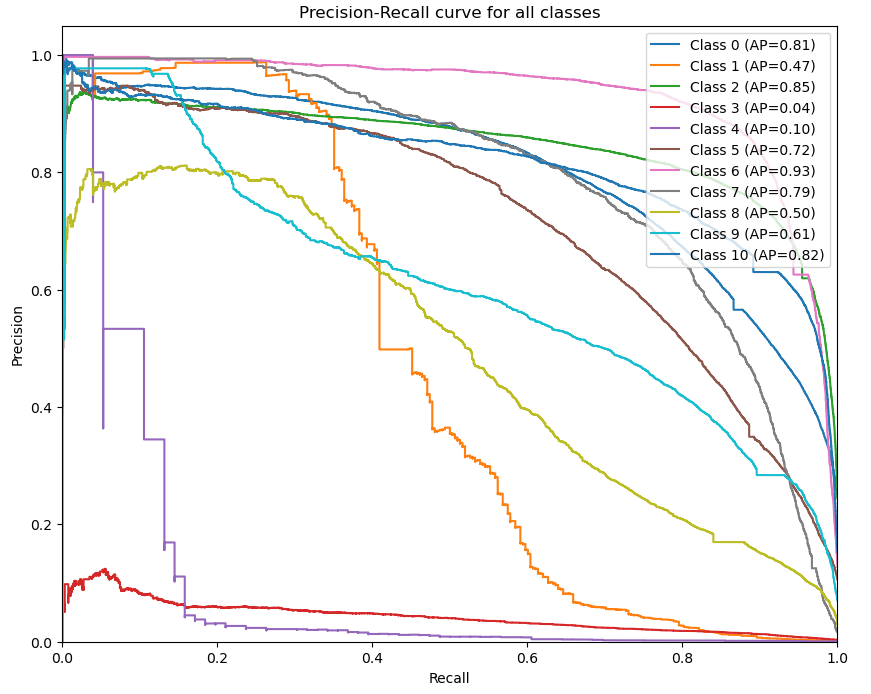
\includegraphics[width=\linewidth]{pr_with_bad.png}
        \caption{PR-кривые для всех классов, ступень 1.5, выборка 1}
        \label{fig:pr1}
    \end{minipage}
    \hfill
    \begin{minipage}[b]{0.54\textwidth}
        \centering
        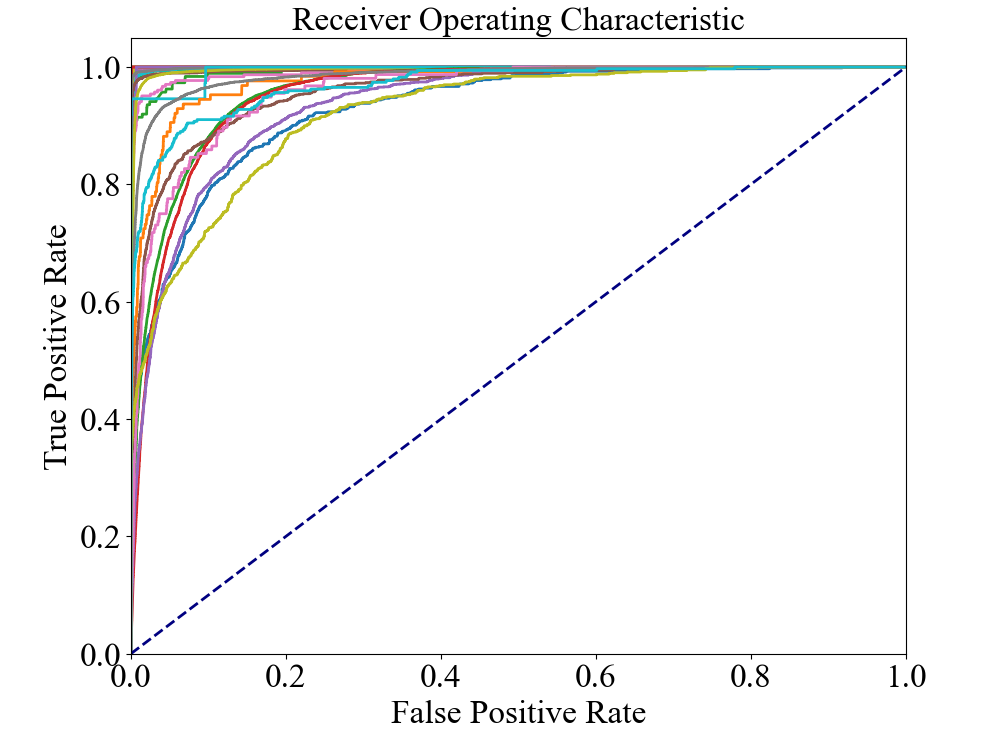
\includegraphics[width=\linewidth]{roc_with_bad.png}
        \caption{ROC-кривые для всех классов, ступень 1.5, выборка 1}
        \label{fig:roc1}
    \end{minipage}
\end{figure}

\begin{itemize}
    \item По результам пункта 5\footnote{Эксперимент и результаты можно посмотреть \href{https://github.com/intsystems/2024-Project-142/blob/master/code/1_17_33_class_full_train-Copy1.ipynb}{тут}}, наблюдаем подтверждение тенденции качественного отделения больших классов и видим улучшение результатов классификации при исключении классов с плохими данными. На рисунке \ref{fig:pr2} - показаны pr-кривые для всех классов ступени 1.5 выборки 2, видим хорошие показатели разделения. 
    \item На рисунке \ref{fig:pr3} - показаны pr-кривые для одного из классов в зависимости от глубины классификации. Видим закономерное ухудшение результата классификации при увеличении ступени, при этом даже на последней ступени результаты удовлетворительные.  
\end{itemize} 


\begin{figure}[!ht]
        \centering
        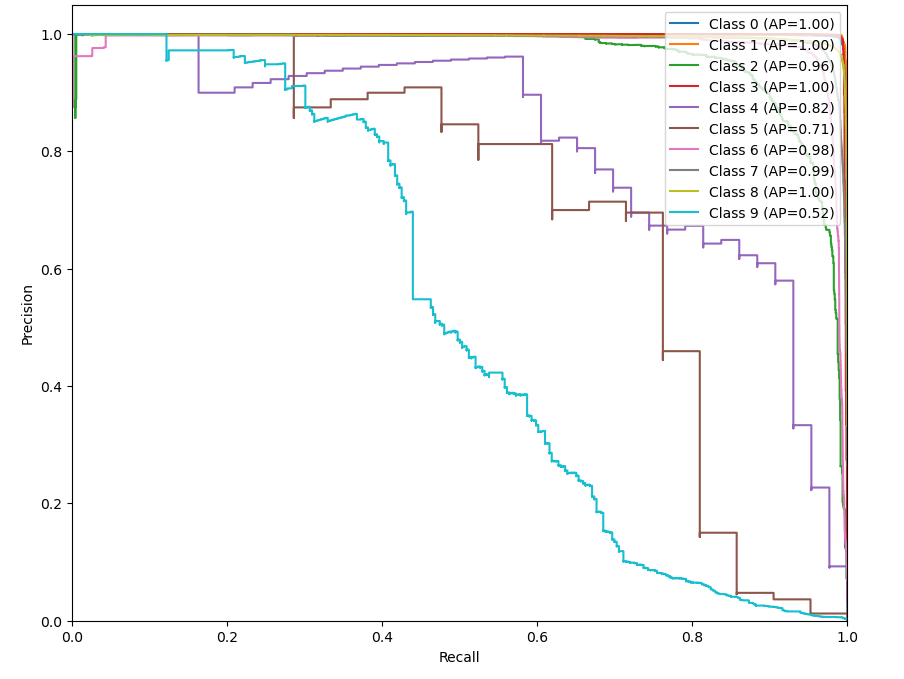
\includegraphics[width=\linewidth]{pr_good.png}
        \caption{PR-кривые для всех классов, ступень 1.5, выборка 2}
        \label{fig:pr2}
\end{figure}
\begin{figure}[!ht]
        \centering
        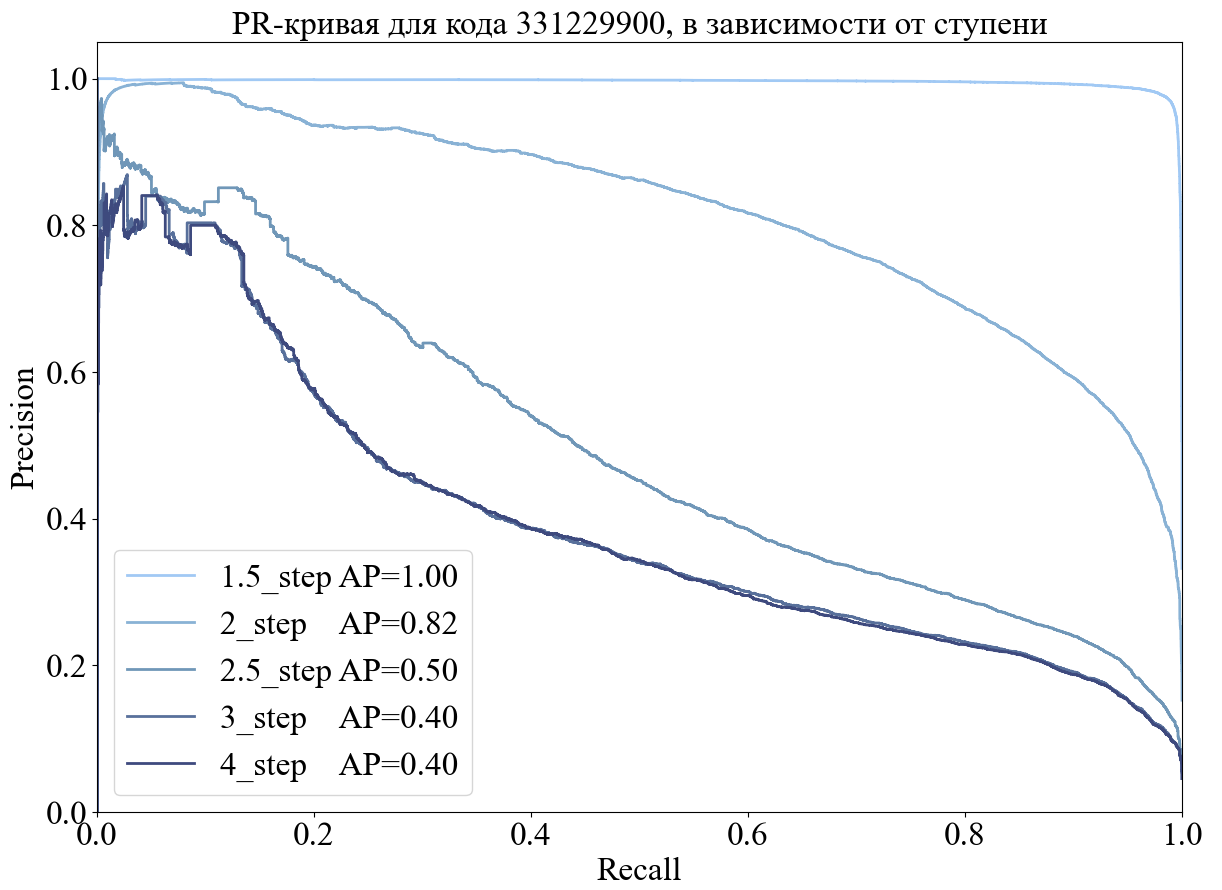
\includegraphics[width=\linewidth]{pr_curve_1.png}
        %\caption{PR-кривые для всех классов, ступень 1.5, выборка 2}
        \label{fig:pr3}
\end{figure}

\begin{itemize}
    \item По результатам экспериментов \footnote{Эксперименты и результаты можно посмотреть \href{https://github.com/intsystems/2024-Project-142/blob/master/code/0_try_ierarhik.ipynb}{тут} и \href{https://github.com/intsystems/2024-Project-142/blob/master/code/0_try_ierarhik.ipynb}{тут}} с проверкой иерархической идеи улучшения классификации получена сводная таблица \ref{tab:1}. В ней показаны количества ошибок (в тысячах), на выборке 2 в зависимости от метода: стандартный, с разбиением выборки на подклассы, с добавлением нового признака. Размер выборки 2 --- 736 тыс. записей.
    
    \begin{table}[ht]
        \centering
        \begin{tabular}{|l|c|c|c|}
            \hline
            \textbf{Метод} & \textbf{Стандартный} & \textbf{С разбиением на подклассы} & \textbf{С добавлением признака} \\ \hline
            Ступень 2 & 90 & \textbf{86} & 87 \\ \hline
            Ступень 2.5 & 106 & \textbf{101} & 103 \\ \hline
            Ступень 3 & 120 & \textbf{112} & 113 \\ \hline
        \end{tabular}
        \caption{Количество ошибок на выборке 2 в зависимости от метода и ступени}
        \label{tab:1}
    \end{table}
    
    \item В таблице \ref{tab:1} наблюдается предполагаемый рост количества ошибок с увеличением номера ступени. Также видим, что предлагаемые методы иерархической классификации улучшают результаты --- наблюдаем уменьшение количества ошибок примерно на 5\%. Чуть лучше себя показывает метод с разбиением на подклассы, как и предполагалось. 
\end{itemize}


\subsection{Выводы}
\begin{itemize}
    \item Модели были построены на различных выборках, и результаты показали, что для крупных классов модель демонстрирует высокую точность, что соответствует целям исследования.
    \item Анализ зависимости качества классификации от глубины классификатора подтвердил ожидаемые тенденции: с увеличением глубины точность падает, но остаётся в приемлемых пределах.
    \item Реализация и тестирование улучшенных методов классификации показали снижение ошибок на 5\%, что подтверждает эффективность предложенных усовершенствований.
\end{itemize}


\section{Заключение}


В рамках данной работы был предложен и реализован алгоритм для классификации товаров по кодам ОКПД2. Разработанная модель основывается на использовании текстовых эмбеддингов и логистической регрессии, что позволило эффективно решать задачу многоклассовой классификации. Было проведено тщательное исследование модели, в ходе которого анализировалось влияние глубины классификатора на качество результатов, а также изучено, как различные гиперпараметры влияют на производительность модели.

Кроме того, в работе были исследованы различные способы улучшения модели, включая модификации алгоритма классификации и применение иерархической структуры классификатора, что позволило улучшить точность классификации, особенно на более глубоких уровнях.

Возможные пути для дальнейших улучшений модели включают:

\begin{itemize}
    \item Улучшение качества текстовых эмбеддингов, возможно, за счет использования более совершенных моделей нейронных сетей или дополнительного дообучения на специфических данных.
    \item Интеграция и усовершенствование предложенных методов улучшения классификации для создания более робустной системы.
    \item Работа над несбалансированностью классов, что может включать техники ресемплинга или специализированные функции потерь.
\end{itemize}


\bibliographystyle{unsrtnat}
\bibliography{Firsov2024Classification_according_to_OKPD_2_codes}

\end{document}